\section{Classification}

\subsection{Behavioral data classification}

The next step in the mini-project was to try and see whether there was a relationship between the three datasets that would allow for behavioral classification.
For this, we used a supervised learning algorithm with the behavioral categories as the discrete target classes.
The algorithm used was a Random Forest Classifier (RFC), as it is not prone to over-fitting, and since decision trees are very simple algorithmically speaking.
An RFC consists of multiple different decision trees merged to get more accurate results.

\vspace{\baselineskip}

The RFC was based on the wavelet angles in order to classify manual behaviors.
We used 25 wavelet features from the joint angles, with frequencies between 1 and \SI{50}{\hertz}.
The resulting classifier displayed an accuracy of around 99.1\% on a test set of the manually predicted data with which it was trained and 77.8\% on the predicted labels column from the initial dataset.
The three most important features in the decision tree were:
\begin{itemize}
	\item the left front leg Coxa roll angle,
	\item followed by the left front leg Coxa pitch angle,
	\item and the left front leg Femur pitch angle.
\end{itemize}

All three features are anatomically located at the base of the fly's leg (see Figure~\ref{fig::drosophila_anatomy}), and probably allow the discrimination between the resting and walking behaviors (the most frequent behaviors). As we are only classyfing behaviors based on joint angles this classifier could be used in other flies.

\begin{figure}[htbp]
	\begin{center}
		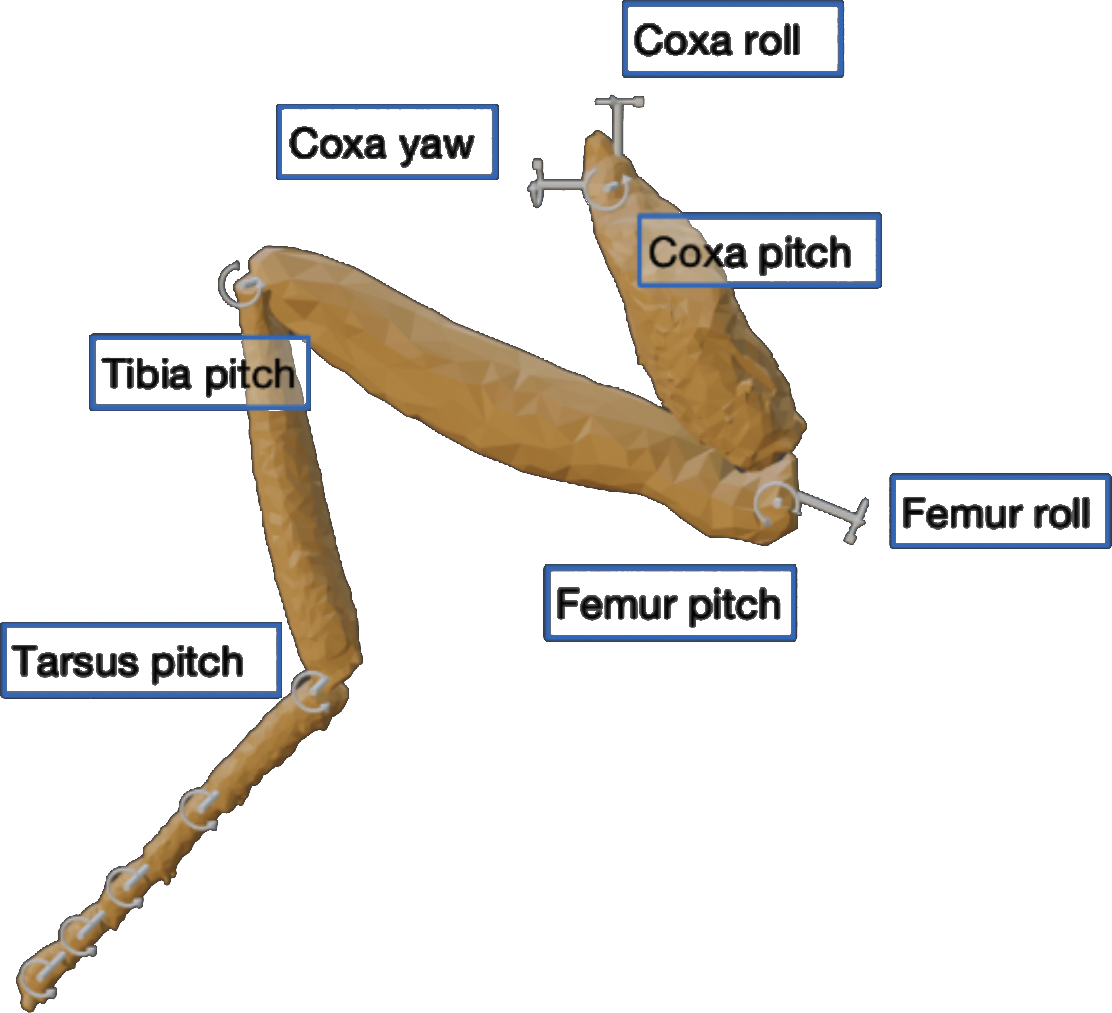
\includegraphics[width=0.4\textwidth]{drosophila_anatomy}
		\caption{The seven joint angles of the \textit{Drosophila} leg segments.}
		\label{fig::drosophila_anatomy}
	\end{center}
\end{figure}

\subsection{Identifying correlations between individual neurons}

In order to try and identify correlation between individual neurons, we normalized the neural dataset to allow comparison between them.
For this we used the z-score.
It corresponds to how many standard deviation from the average a single sample of the signal is.

\vspace{\baselineskip}

After having standardized the neuronal data, we first computed the average activity in all neurons during the different behaviors to see whether some behaviors were triggering higher or lower activity in the neurons. But as can be seen on Figure~\ref{fig::mean_neuron_behav_matrix}, this is not the case. 

\begin{figure}[htbp]
	\begin{center}
		\includesvg[width=0.7\textwidth]{mean_neuron_behav_matrix}
	\end{center}
	\caption{Box plot of average activity for all neurons across the different behaviors.}
	\label{fig::mean_neuron_behav_matrix}
\end{figure}

Then, in order to have a visual representation of specific neural activity, we plotted a matrix of the neurons and their activity levels, which is displayed on Figure~\ref{fig::neuron_behav_matrix}.

\begin{figure}[htbp]
	\begin{center}
		\includesvg[width=0.7\textwidth]{neuron_behav_matrix}
	\end{center}
	\caption{Matrix of the neurons and their relative activity across the different behaviors.}
	\label{fig::neuron_behav_matrix}
\end{figure}

The matrix does not give much insight about a possible higher neural activity given a specific behavior.
Although we can see some higher activity in neurons for certain behaviors, we cannot conclude anything from the matrix.

This prompted us to us to turn towards statistical tools to try and discover correlation between behavior and neural activity.

\vspace{\baselineskip}

For this we used an ANOVA test combined with a Tukey test.
The ANOVA test is a generalization of the t-test, and measures whether two or more distributions have similar means or not.
This is useful for the behavioral data, because there are more than two behavioral categories.

\vspace{\baselineskip}

After the analysis of variance, we tested whether the difference between two behaviors was significant at a 5\% level with a Tukey test.
This test takes the ANOVA significant output and finds out which specific distributions are different by comparing all possible pairs.
The goal was to look for neurons that, for a given behavior, have a significantly different activity than with all other behaviors, at a 5\% level.
The results presented in Table~\ref{tab::statistical_table} are those of such neurons, with the respective associated behavior.

\begin{table}[htbp]
	\sffamily
	\arrayrulecolor{white}
	\arrayrulewidth=1pt
	\renewcommand{\arraystretch}{1.5}
	\rowcolors[\hline]{1}{.!50!White}{}
	\centering
	\begin{tabular}{@{} B|A @{}}
		\cellcolor{ForestGreen}\arraycolor{White}\bfseries Neuron &
		\cellcolor{ForestGreen}\arraycolor{White}\bfseries Behavior \\   
		\arraycolor{Black}
		2 & resting \\
		3 & resting \\
		62 & resting \\
		80 & resting \\
		81 & resting \\
		25 & foreleg grooming \\
		36 & foreleg grooming \\
		42 & abdominal pushing \\
		71 & abdominal pushing \\
		86 & abdominal pushing \\
		109 & abdominal pushing \\
		122 & abdominal pushing \\
		113 & antennal pushing \\
		122 & abdominal grooming \\
	\end{tabular}
	\caption{Neurons exhibiting a significant difference in activity compared with the other neurons when the fly performs the specified associated behavior.}
	\label{tab::statistical_table}
\end{table}

With these results, the next step is to group them by significant behavior, and plot them against time, like on Figures~\ref{fig::trial_7_resting} and~\ref{fig::trial_7_antennal_grooming}.

\begin{figure}[htbp]
	\begin{center}
		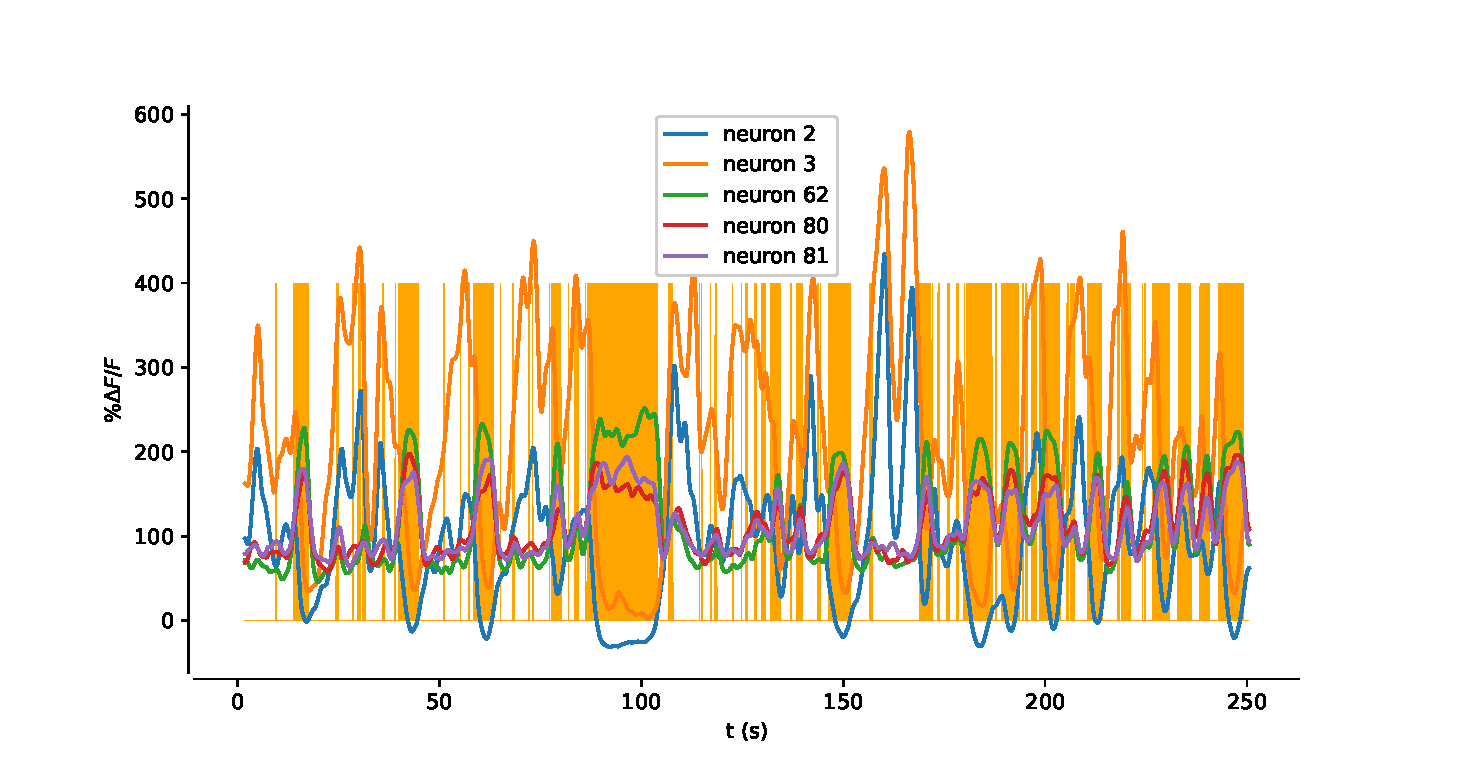
\includegraphics[width=\textwidth]{trial_7_resting}
	\end{center}
	\caption{Neural activity for trial 7, resting state in orange overlay.}
	\label{fig::trial_7_resting}
\end{figure}

\begin{figure}[htbp]
	\begin{center}
		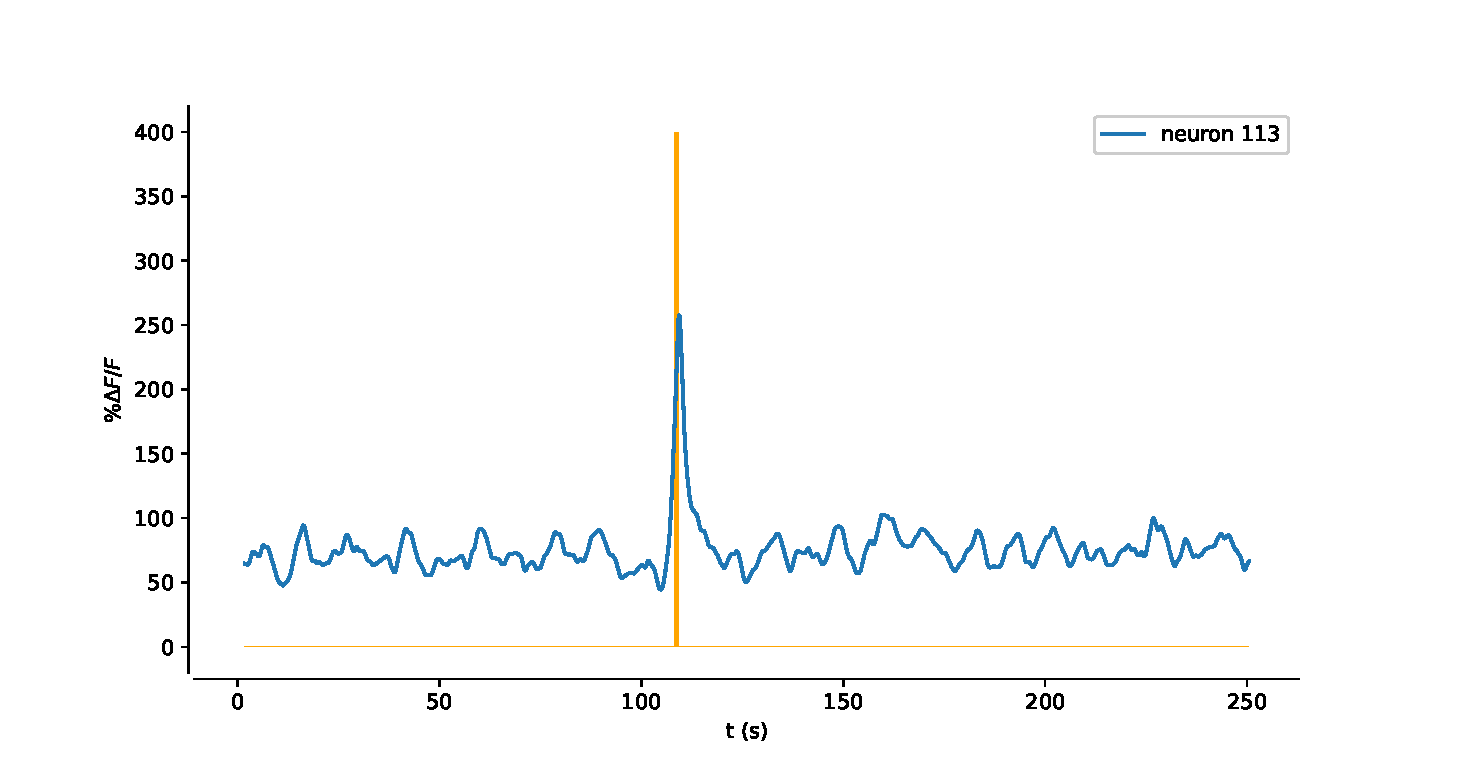
\includegraphics[width=\textwidth]{trial_7_antennal_grooming}
	\end{center}
	\caption{Neuron 113 activity for trial 7, antennal grooming state in orange overlay.}
	\label{fig::trial_7_antennal_grooming}
\end{figure}

We already saw that several behaviors are seldom exhibited by the fly.
This means that the respective data risks being sparse.
For example, for the walking behavior, 58 out of the 123 neurons exhibit a significantly different activity than for the other behaviors, except for hind leg grooming.
However, hind leg grooming is a comparatively rare behavior, that happens only twice in the downsampled behavioral dataset.
Thus, if it were removed from the analysis, the walking behavior could be taken into account.
Here, analyzing 58 additional neurons individually might not be the most effective method, so they were still excluded from Table~\ref{tab::statistical_table}.
The 58 neurons concerned are neurons 2, 5, 7, 9, 10, 11, 12, 20, 21, 23, 25, 26, 29, 30, 31, 32, 34, 36, 38, 39, 41, 48, 49, 51, 55, 58, 59, 61, 62, 63, 65, 68, 69, 70, 71, 73, 76, 78, 79, 82, 85, 86, 89, 91, 92, 94, 95, 97, 99, 101, 102, 105, 106, 114, 116, 117, 121 and 122.

\vspace{\baselineskip}

Then, the Spearman's correlation coefficient between neural data and joint angles was studied.
Joint angles were selected as opposed to joint position, because it was shown earlier that there they are more important for behavioral analysis.
Spearman's correlation coefficient is a method that aims to find a statistical dependence between the ranking of two variables.
In Table~\ref{tab::spearman_table}, the Spearman's correlation coefficients greater than 0.5 or lesser than -0.5 are retained, to observe moderately to highly correlated joint angles to neural data, keeping only the ones where the p-value of that correlation was lower than 5\%.

\begin{table}[htbp]
	\sffamily
	\arrayrulecolor{white}
	\arrayrulewidth=1pt
	\renewcommand{\arraystretch}{1.5}
	\rowcolors[\hline]{1}{.!50!White}{}
	\centering
	\begin{tabular}{@{} B|A|A @{}}
		\cellcolor{ForestGreen}\arraycolor{White}\bfseries Neuron &
		\cellcolor{ForestGreen}\arraycolor{White}\bfseries Angle &
		\cellcolor{ForestGreen}\arraycolor{White}\bfseries Correlation \\   
		\arraycolor{Black}
		36 & LM leg Femur & 0.63 \\
		25 & LM leg Femur & 0.61 \\
		101 & RH leg Coxa roll & 0.58 \\
		117 & LM leg Femur & 0.57 \\
		65 & LM leg Femur & 0.55 \\
		102 & LM leg Femur & 0.55 \\
		63 & LM leg Femur & 0.55 \\
		25 & LF leg Femur & 0.50 \\
		36 & RM leg Femur & 0.50 \\
		36 & LF leg Femur & 0.50 \\
		36 & LM leg Tarsus & -0.57 \\
		25 & LM leg Tarsus & -0.57 \\
		25 & RH leg Coxa roll & -0.55 \\
		102 & RH leg Coxa roll & -0.52 \\
		20 & RH leg Coxa roll & -0.52 \\
		117 & LM leg Tarsus & -0.51 \\
		36 & RM leg Tarsus & -0.50 \\
	\end{tabular}
	\caption{Spearman's correlation coefficients for correlated joint angles with the neural data.}
	\label{tab::spearman_table}
\end{table}

On Figure~\ref{fig::spearman_neuron_36} is plotted the biggest Spearman's correlation coefficient, which is for neuron 36 and the left medial Femur angle, with a coefficient of 0.63, $p<0.05$.

\begin{figure}[htbp]
	\begin{center}
		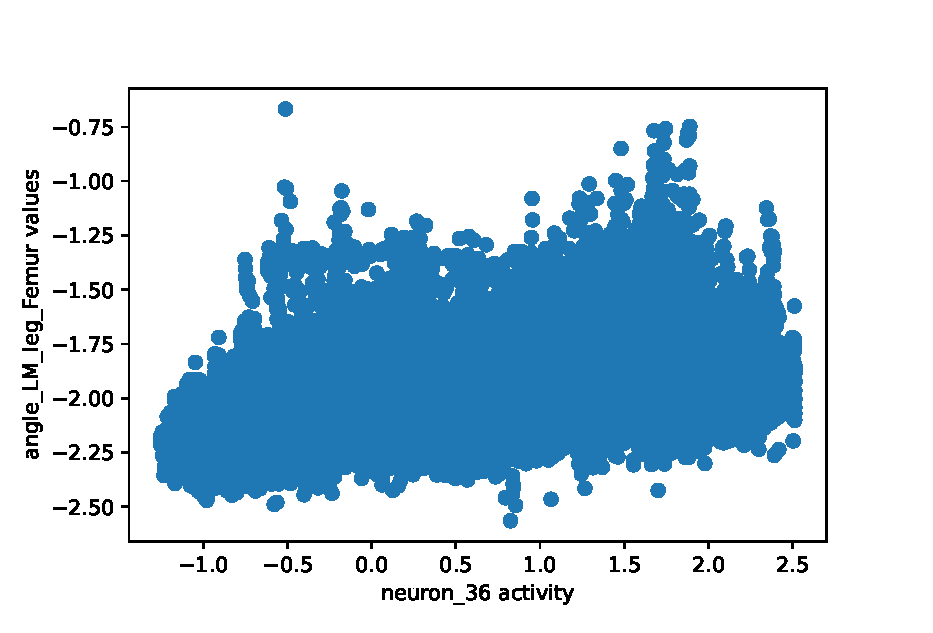
\includegraphics[width=0.6\textwidth]{spearman_neuron_36}
	\end{center}
	\caption{Spearman's positive correlation coefficient of 0.63, $p<0.05$ for neuron 36 for the left medial Femur.}
	\label{fig::spearman_neuron_36}
\end{figure}

The highest correlation is not very high.
A possible explanation is that DNs are more correlated to behavioral categories than to joint angles.
From a neural and anatomical perspective, it could be explained if those neurons encode entire behaviors rather than joint angles, the latter being a result in a process involving many different neuron contributions. 

\subsection{Predicting behavior from neural activity}

\subsubsection{Logistic regression with one behavior: walking}

Then, a logistic regression was performed on the neural data points in order to classify behaviors.
Logistic regression is a method that classify binary categorical outputs, e.g. walking or not walking.
It is based on a logistic function that smoothly varies from 0 to 1 depending on the input. 
The first logistic regression done was performed on each neural activity separately as input, with the output being whether or not the fly exhibit the walking behavior. Table~\ref{tab::lr_single_neuron} summarizes the results of the regression with the 10 most predictive neurons with their maximum accuracy.

\begin{table}[htbp]
	\sffamily
	\arrayrulecolor{white}
	\arrayrulewidth=1pt
	\renewcommand{\arraystretch}{1.5}
	\rowcolors[\hline]{1}{.!50!White}{}
	\centering
	\begin{tabular}{@{} B|B @{}}
		\cellcolor{ForestGreen}\arraycolor{White}\bfseries Neuron &
		\cellcolor{ForestGreen}\arraycolor{White}\bfseries Accuracy \\   
		\arraycolor{Black}
		32 		& 0.788		\\
		38		& 0.787		\\
		99		& 0.785		\\
		28 		& 0.784 	\\
		12 		& 0.779 	\\
		51		& 0.774		\\
		93		& 0.773		\\
		62		& 0.772		\\
		48		& 0.771 	\\
		5		& 0.768		\\
		All 	& 0.853
	\end{tabular}
	\caption{Logistic regression accuracy for the 10 most accurate neurons for the walking behavior.}
	\label{tab::lr_single_neuron}
\end{table}

Table~\ref{tab::lr_single_neuron} shows that looking for the specific neurons that best classify for the walking behavior provides us with approximately 40 with an accuracy greater than 70\%.
If instead of looking for a specific neuron, we look at all the neurons together, we can classify for the walking behavior with an accuracy of 85\%.
This let's us think that the walking behavior is not controlled by only one neuron, but several, which is consistent with the results of the ANOVA.

\vspace{\baselineskip}

On Figures~\ref{fig::ow_neuron_32} and~\ref{fig::ow_neuron_38} are displayed the two most relevant neurons found in Table~\ref{tab::lr_single_neuron}.
For both, there is a definite increase in neural activity during the walking motion, and a definite decrease in activity during resting.

\subsubsection{Logistic regression with multiple behaviors}

The logistic regression was then applied to all neural activity in order to classify all the neurons.
The accuracy found for this regression is 0.806.
Table~\ref{tab::lr_multiple_neuron} summarizes the 10 most important neurons for each behavior.

\begin{table}[htbp]
	\sffamily
	\arrayrulecolor{white}
	\arrayrulewidth=1pt
	\renewcommand{\arraystretch}{1.5}
	\rowcolors[\hline]{1}{.!50!White}{}
	\centering
	\begin{tabular}{@{} A|C|C|C|C|C|C|C|C|C|C @{}}
		\cellcolor{ForestGreen}\arraycolor{White}\bfseries Neuron &
		\cellcolor{ForestGreen}\arraycolor{White}\bfseries 1 &
		\cellcolor{ForestGreen}\arraycolor{White}\bfseries 2 &
		\cellcolor{ForestGreen}\arraycolor{White}\bfseries 3 &
		\cellcolor{ForestGreen}\arraycolor{White}\bfseries 4 &
		\cellcolor{ForestGreen}\arraycolor{White}\bfseries 5 &
		\cellcolor{ForestGreen}\arraycolor{White}\bfseries 6 &
		\cellcolor{ForestGreen}\arraycolor{White}\bfseries 7 &
		\cellcolor{ForestGreen}\arraycolor{White}\bfseries 8 &
		\cellcolor{ForestGreen}\arraycolor{White}\bfseries 9 &
		\cellcolor{ForestGreen}\arraycolor{White}\bfseries 10 \\   
		\arraycolor{Black}
		Resting 				& 0 & 62 & 109 & 48 & 100 & 101	& 73 & 30 & 41 & 36 \\
		Walking					& 28 & 109 & 100 & 103 & 117 & 48 & 101 & 23 & 39 & 38 \\
		Abdominal pushing		& 22 & 7 & 8 & 20 & 40 & 116 & 105 & 30 & 23 & 42 \\
		Anterior grooming 		& 34 & 89 & 99 & 84 & 44 & 38 & 100 & 51 & 65 & 119 \\
		Posterior grooming 		& 118 & 120 & 47 & 33 & 43 & 112 & 108 & 39 & 93 & 89 \\
		Foreleg grooming		& 85 & 89 & 51 & 61 & 44 & 102 & 2 & 99 & 0 & 81 \\
		Abdominal grooming		& 50 & 87 & 43 & 83 & 7 & 107 & 60 & 52 & 90 & 95 \\
		Hind leg grooming		& 27 & 74 & 9 & 122 & 76 & 107 & 22 & 98 & 58 & 93 \\
		Antennal grooming		& 99 & 21 & 34 & 89 & 41 & 34 & 91 & 103 & 65 & 32 \\
	\end{tabular}
	\caption{The ten most accurate neurons for each behavior from logistic regression accuracy.}
	\label{tab::lr_multiple_neuron}
\end{table}

It can be seen on Table~\ref{tab::lr_multiple_neuron} that a lot of neurons found in the walking behavior classification are also overall important for the classification when taking into account all behaviors, like for example neurons 38 and 28.

\vspace{\baselineskip}

On Figures~\ref{fig::ow_neuron_32},~\ref{fig::ow_neuron_38},~\ref{fig::fr_neuron_93} and~\ref{fig::rf_neuron_62}, the neural activity was plotted with the resting and walking states in overlay. As already stated, for each there is a definite increase in neural activity during the walking motion, and a definite decrease in activity during resting.

\begin{figure}[hbtp]
	\begin{center}
		\includesvg[width =\textwidth]{neuron_32}
	\end{center}
	\caption{Neuron 32 activity, resting state in orange overlay, walking state in blue overlay.}
	\label{fig::ow_neuron_32}
\end{figure}

\begin{figure}[hbtp]
	\begin{center}
		\includesvg[width =\textwidth]{neuron_38}
	\end{center}
	\caption{Neuron 38 activity, resting state in orange overlay, walking state in blue overlay.}
	\label{fig::ow_neuron_38}
\end{figure}

\begin{figure}[hbtp]
	\begin{center}
		\includesvg[width =\textwidth]{neuron_93}
	\end{center}
	\caption{Neuron 93 activity, resting state in orange overlay, walking state in blue overlay.}
	\label{fig::fr_neuron_93}
\end{figure}

\begin{figure}[hbtp]
	\begin{center}
		\includesvg[width =\textwidth]{neuron_62}
	\end{center}
	\caption{Neuron 62 activity, resting state in orange overlay, walking state in blue overlay.}
	\label{fig::rf_neuron_62}
\end{figure}

It can be observed on these Figures that neural activity is a very good predictor for the walking and resting behaviors.

\subsubsection{Random forest classifier}

To compare the results found with the logistic regression, a random forest classifier was trained.
It was found to have an accuracy of 87.5\%.
The ten most important neurons for the classifier are neurons 93, 62, 60, 103, 28, 81, 29, 23, 51 and 32.

\newpage

